The observation of the NS merger GW170817 has provided for the first time the empirical
estimate of the tidal deformation of NS induced by strong gravitational field between 
the two companions of a merging binary pulsar \citep{hinderer2008tidal,hinderer2010tidal}. In this chapter, 
we discuss briefly, within the frame of General Relativity, how a static spherical NS can be
tidally deformed by gravitation, gaining nonzero gravito-multipole moments which are
directly proportional to the strength of gravitation \citep{damour2009relativistic}.
The tidal deformation moments of different multipoles are determined in the present work 
with the mean-field based EoS of spin-polarized NS matter using the explicit expressions 
of the Love numbers given by GR \citep{perot2021role}. The obtained results for the tidal
deformability as well as the gravitational mass $M$ and radius $R$ of \gls{NS} are 
compared in details with the astrophysical constraints deduced from the observation 
of GW170817.

\section{Einstein equations of relativistic neutron star}%
\label{sec3}
In general, the line element of metric in the static isotropic spacetime can be 
expressed within GR  \citep{glendenning2012compact} in terms of spatial spherical 
coordinates as
\begin{equation}
        ds^2 = g_{\mu\nu}dx^\mu dx^\nu=e^{2\nu(r)}c^2dt^2 - e^{2\lambda(r)}dr^2 - 
				r^2 d\theta^2 - r^2\sin^2\theta d\phi^2, \label{metr}
\end{equation}
where arbitrary functions $\nu(r)$ and $\lambda(r)$ are determined locally by the
mass-energy density enclosed within the sphere of radius $r$. In the vicinity of a 
static spherical NS, the spacetime geometry is determined from the pressure and 
mass-energy density of NS matter (treated as a perfect fluid), and the  
energy-momentum tensor is obtained in \gls{GR} as
\begin{equation}
        T^{\mu\nu}=- Pg^{\mu\nu} + (P+\rho) u^\mu u^\nu,\ 
				g_{\mu\nu}u^\mu u^\nu=u_\nu u_\nu=1.
\end{equation}
Here $P$ and $\rho$ are the pressure and mass-energy density of NS matter, respectively,
$u^\mu = dx^\mu/d\tau$ is the local fluid 4-velocity. The Einstein's field 
equations of neutron star are written as 
\begin{equation}
        G^{\mu\nu} = - \frac{8\pi G}{c^4} T^{\mu\nu}. \label{Ein} 
\end{equation}
Keeping the nonrelativistic limit to the static Newtonian gravitation, the 
Einstein's field equations (\ref{Ein}) can be reduced to the following differential 
equations which are known as Tolman-Oppenheimer-Volkoff (\gls{TOV}) equations 
\citep{glendenning2012compact}
\begin{eqnarray}
\frac{d P(r)}{dr}&=& -\frac{G \rho(r)\mathcal{M}(r)}{c^2 r^2} 
 \left[ 1+\frac{P(r)}{\rho(r)}\right] 
\left[1+\frac{4 \pi P(r) r^3}{c^2 \mathcal{M}(r)} \right] 
\left[ 1-\frac{2G \mathcal{M}(r)}{c^2 r} \right]^{-1}, \nonumber \\
d\mathcal{M}(r) &=& 4\pi r^2 \rho(r)dr, \label{tov} 
\end{eqnarray}
where $r$ is the radial coordinate in Schwarzschild metric (\ref{metr}), and 
$\mathcal{M}(r)$ is the gravitational mass enclosed within sphere of radius $r$. 
$\rho(r)$ and $P(r)$ are the mass-energy density and pressure of NS matter at 
distance $r$ from the star center, respectively. TOV equations (\ref{tov}) are 
integrated from $r=0$ to the surface of NS, with the star radius $R$ given by 
$P(R)=0$. Other boundary conditions are 
\begin{align}
\mathcal{M}(0)=0, \quad \rho(0)=\rho_{\rm c}, \quad P(0)=P_{\rm c},\quad \mathcal{M}(R)=M.   
\end{align}
The solutions of the TOV equations \eqref{tov} obtained with the given \gls{EoS}
of NS matter readily give the density profiles of the mass and pressure of 
\gls{NS} matter as functions of distance $r$ from the star center. The total mass 
$M$ and radius $R$ of NS can be obtained from the profiles of central pressure 
$P_{\rm c}$ and mass-energy density $\rho_{\rm c}$.

\begin{figure}[ht!]
    \centering
    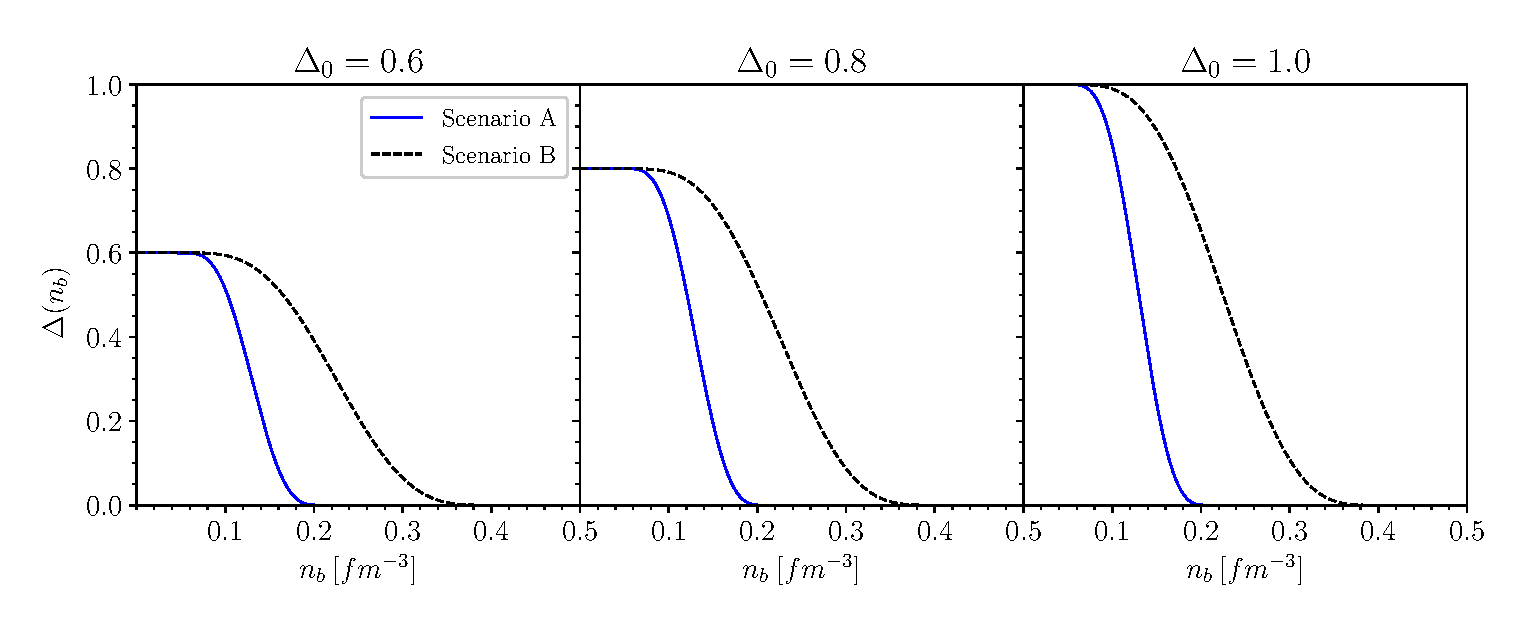
\includegraphics[width=\textwidth]{fig/Delta.eps}
    \caption{Scenarios of the density-dependence of the baryon spin polarization at 3 levels of $\Delta_0$.}
    \label{fig:Delta}
\end{figure} 
Beside, due to the complexity of the magnetic field distribution inside a magnetar \citep{fujisawa2014magnetic}, a density-independent $\Delta$ of \gls{NS} matter does not fully reflect the reality. Particularly, in the inner core of the magnetar, baryons are heavily compressed at extremely high density by gravity, which leads to the full degeneracy, i.e. all possible quantum states are occupied, of baryons in this region and there is no room for baryon to change its spin orientation. Along with the magnetic field, the spin polarization of baryon is expected to gradually weaken to $\Delta \approx 0$ the nearer to the stellar center, in other words, at higher density \citep{fujisawa2014magnetic,tan2020spin}. Although it's beyond the scope of the current study to precisely calculate the density-dependence of $\Delta(n_b)$, we will explore such effect by investigating different scenarios proposed by \cite{tan2020spin} based on the magnetic field distribution of magnetar modelled by \cite{fujisawa2014magnetic}, i.e.
\begin{enumerate}[label=(\Alph*)]
    \item The magnetic field is strongly localized in the surface region of the magnetar, near the crust-core transition, and falls to $B\approx 0$ at $n_b \approx 0.18\: fm^{-3}$,
    \item The magnetic field distribution is broader and decreases gradually to zero at a denser region, which cover both the crust and the outer core, of $n_b \approx 0.35\:fm^{-3}$.
\end{enumerate}
Each scenario was considered with $\Delta_0 = \Delta(n_b \approx 0)$ at the value of partial polarization $\Delta_0 = 0.6$, $0.8$ and total polarization $\Delta_0 = 1.0$ as shown in Figure \ref{fig:Delta}

\begin{figure}[ht!]
        \centering
        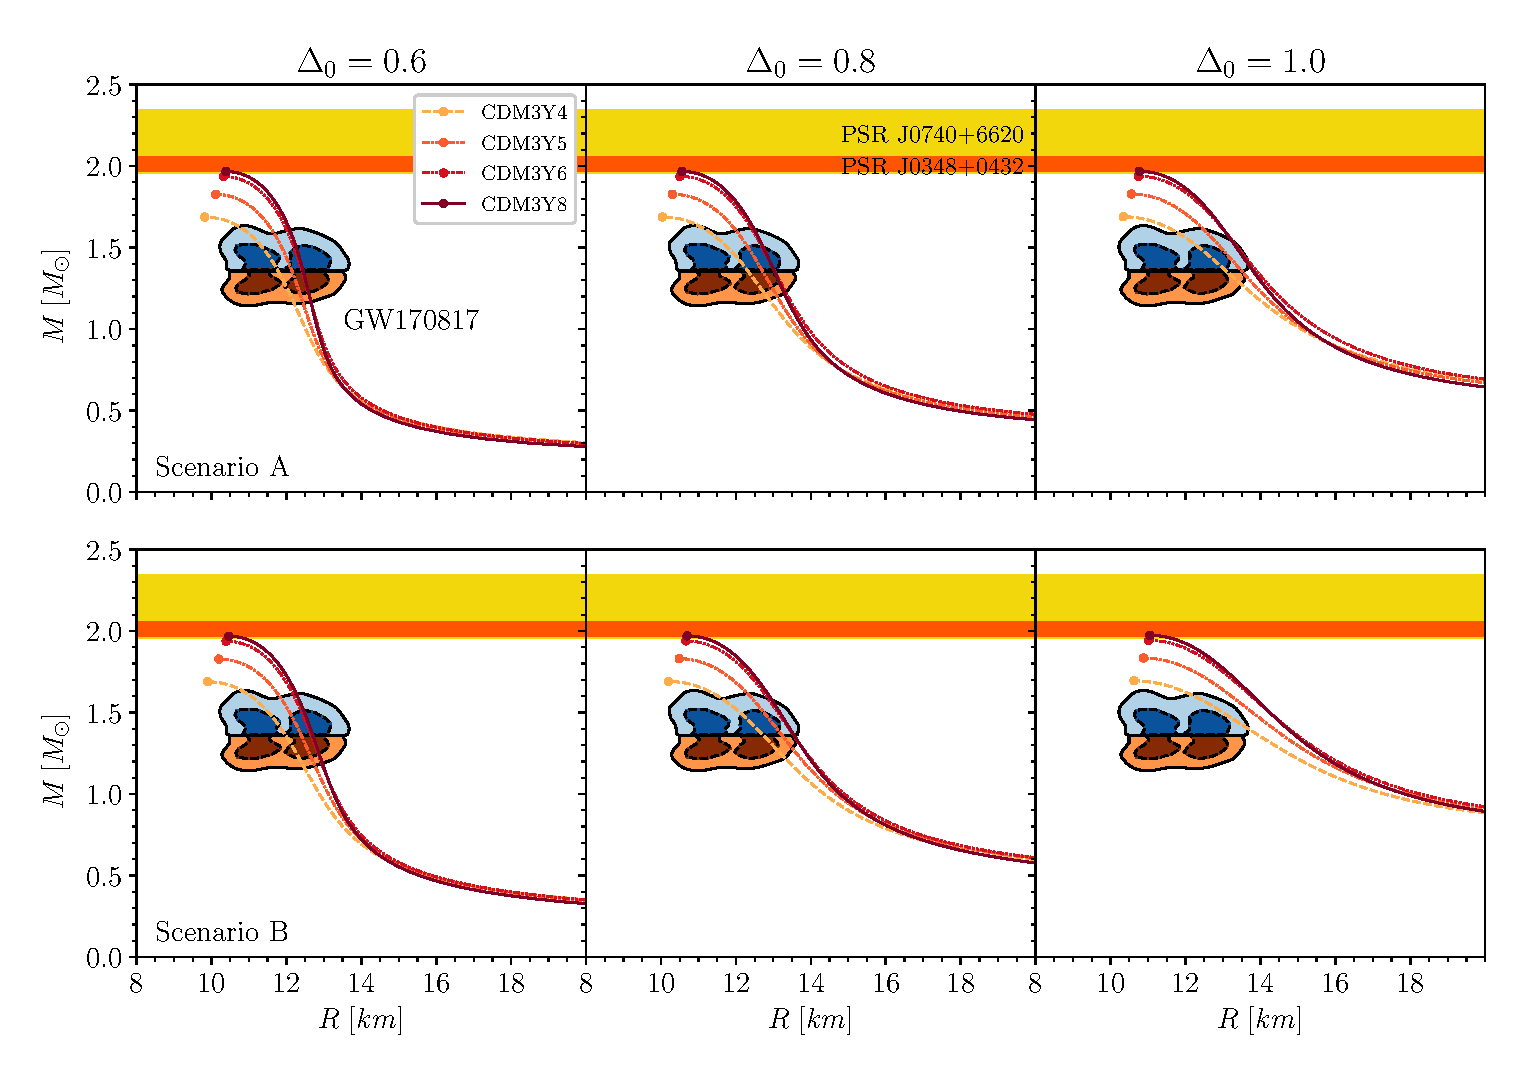
\includegraphics[width=\textwidth]{fig/MR.eps}
        \caption{The relation between gravitational mass $M$ and the radius $R$ of the magnetar according to the corresponding model and polarization. The GW170817 constraint for \gls{NS} with mass $1.4M_\odot$ is shown by the colored contour, where the blue (red) shaded area represents the heavier (lighter) \gls{NS} \citep{abbott2018gw170817}. The dot in each line indicates the maximum \gls{NS} mass of the each model. The dark and light orange region indicates the mass of the second \gls{PSR} J0348+0432 \citep{antoniadis2013massive} and millisecond \gls{PSR} J0740+6620 \citep{cromartie2020relativistic} respectively.}
        \label{fig:mr}
\end{figure} 
With each \gls{NN} interaction, a \textbeta-stable $npe\mu$ matter is generated, which in turn traces a $M(R)$ relation of the respective \gls{NS} for every different $\Delta(n_b)$ configuration, which are shown in Figure \ref{fig:mr} in comparison with the GW170817 constraint \citep{abbott2018gw170817}, as well as the lower mass limit of the second \gls{PSR} J0348+0432 ($M\approx 2.01^{+0.04}_{-0.04}M_\odot$) and the millisecond \gls{PSR} J0740+6620 ($M\approx 2.14^{+0.20}_{-0.18}M_\odot$), i.e. the heaviest \glsplural{NS} observed so far. Notably, it is interesting that all 4 versions of the interaction here remain inside the empirical range at $M=1.4M_\odot$ at $\Delta_0 = 0.6$ and the scenario A when $\Delta_0 = 0.8$; the configurations with $\Delta_0 = 1.0$, unsurprisingly, give unsatisfying result, similar to the conclusion reached by \cite{tan2020spin} and \cite{tews2020spin}. The radius of a $1.4M_\odot$ \gls{NS} at $\Delta_0 = 0.6$ in the surface of the magnetar is found to be $\approx 11.2 - 12.7\:km$ with scenario A, which is in agreement with the empirical value $R_{1.4} \approx 11.75^{+0.86}_{-0.81}M_\odot$ deduced from the joint analysis of two \gls{GW} events GW170817 and GW190425 from two different \gls{NS} mergers \citep{dietrich2020multimessenger}, and the more polarized the \gls{NS} matter, the larger the \gls{NS} generated is, similar to the result of \cite{tan2020spin}. Apart from the radius, the maximum mass of the \gls{NS} corresponding to each \gls{EoS} has no significant change from scenario to scenario and from the occurence of magnetic field in the magnetar surface \citep{tan2021equation}. Beside, the observation of two heaviest pulsars \gls{PSR} J0348+0432 and \gls{PSR} J0740+6620 gives us more information to further investigate the the \gls{EoS}'s sensitivity to the value of $K$ and $\Delta(n_b)$; in particular, among the 4 interaction versions that satisfy the GW170817 constraint (the case of $\Delta_0 = 0.6$), only the CDM3Y6 and CDM3Y8 interactions come close to the lower limit of these two pulsars' mass.

\section{Gravito-electric and gravito-magnetic deformability}%
\label{sec:gravito_electric_and_gravito_magnetic_deformability}

Here we give a brief review on the theory of gravitoelectromagnetism (\gls{GEM}), as presented by \cite{mashhoon2003gravitoelectromagnetism} and \cite{damour2009relativistic}, starting from the linear perturbation approach. In a binary system of \glsplural{NS}, due to powerful gravitational effects caused by the companion, the global background inertial frame $x^{\mu} = (ct, \mathbf{x})$ and Minkowski metric $\eta_{\mu\nu}$ is perturbed to linear order, i.e.
\begin{equation}
    g_{\mu\nu} \approx \eta_{\mu\nu} + h_{\mu\nu}(x)
\end{equation}
With such perturbed metric tensor, the Einstein's field equation \eqref{Ein} reads
\begin{equation}
    \square \bar{h}_{\mu\nu} = - \frac{16\pi G}{c^4} T_{\mu\nu} \label{Ein_pert}
\end{equation}
where $\bar{h}_{\mu\nu} = h_{\mu\nu} - \frac{1}{2} \eta_{\mu\nu}\eta^{\rho\sigma}h_{\rho\sigma}$. Remarkably, the equation \eqref{Ein_pert} is completely analogous to the well known Maxwell's equations of classical electromagnetism
\begin{equation}
    \square A^\nu = 4\pi j^\nu
\end{equation}
with $A$ being the electromagnetic field strength tensor and $j$ being the current 4-vector. By introducing the \gls{GEM} potentials $\Phi$ and $\mathbf{A}$ as $\bar{h}_{00}=4\Phi/c^2$ and $\bar{h}_{0i} = -2A_i/c^2$, we define the \gls{GEM} fields as
\begin{equation}
    E_{i} = 4\partial_i\Phi + \frac{2}{c} \pdv{A_i}{t},\quad B_i = -2c\epsilon_{ijk}\partial_j A_k
\end{equation}
Note that these definitions differ from those in \cite{mashhoon2003gravitoelectromagnetism} by a factor of $-2$ (or $-2c$) in order to coincide with the definitions used by \cite{damour2009relativistic} for the study of \gls{NS}'s tidal properties. Plus, in the Newtonian limit, the \gls{GE} potential reduces to $\sim GM/r$, which is the classical gravitational potential. Analogous to the classical theory of electromagnetism, the tidal field experienced by it can be decomposed into 2 types: the \emph{gravito-electric} (\gls{GE}) and \emph{gravito-magnetic} (\gls{GM}) components with respective \emph{relativistic tidal moment} \citep{damour2009relativistic}
\begin{equation}
        \mathcal{E}_L = \partial_{L-1} E_{a_l} \qquad\text{and}\qquad \mathcal{B}_L = \partial_{L-1} B_{a_l}
\end{equation}
where $E_{a_l}$ and $B_{a_l}$ are the $a_l$ component of the externally generated local \gls{GE} and \gls{GM} field, $L$ represents the multi-index $(a_1, a_2,\ldots, a_l)$ and $l$ being the order of the moment. As a result, the deformation of \gls{NS} is parameterized by the \gls{GE} and \gls{GM} \emph{tidal deformabilities} $\lambda_l$ and $\sigma_l$, i.e. in leading order \citep{damour2009relativistic}
\begin{IEEEeqnarray}{rCl}
    \mathcal{Q}_L &=& \lambda_l \mathcal{E}_L,\label{ge}\\
    \mathcal{S}_L &=& \sigma_l \mathcal{B}_L\label{gm}
\end{IEEEeqnarray}
with $\mathcal{Q}_L$ being the induced mass multipole moment, i.e. the deviation of the mass distribution from spherically symmetry at order $l$, while $\mathcal{S}_L$ is the current multipole moment in adiabatic approximation \citep{damour2009relativistic,perot2021role}. The equations \eqref{ge} and \eqref{gm} give a direct link between the tidal field strengths and the multipole moments of the object, in which the reaction of the body is directly propertional to the field strengths. Plus, it is evident that the higher $\lambda_l$ (or $\sigma_l$) is, the stronger the \gls{NS} deforms under the same tidal field. From these deformabilities, the dimensionless \gls{GE} and \gls{GM} \emph{tidal Love numbers} are defined as \citep{perot2021role}
\begin{equation}
        k_l = \frac{1}{2} (2l-1)!! \frac{G\lambda_l}{R^{2l+1}} \quad \text{and}\quad j_l = 4(2l-1)!! \frac{G\sigma_l}{R^{2l+1}} 
\end{equation}
These parameters are directly related to the \gls{GE} and \gls{GM} \emph{tidal deformability parameters} as
\begin{IEEEeqnarray}{rCl}
    \Lambda_l &=& \frac{2}{(2l-1)!!} k_l \left( \frac{c^2 R}{GM} \right)^{2l+1} \label{eq:Lambda}\\
    \Sigma_l &=& \frac{1}{4(2l-1)!!} j_l \left( \frac{c^2 R}{GM} \right)^{2l+1}
\end{IEEEeqnarray}
which can be extracted from the signal of \gls{GW}. In order to properly calculate these parameters, let $H_l(r)$ and $\tilde{H}_l(r)$ characterize small perturbations of the static metric. These functions have to satisfy \citep{perot2021role,damour2009relativistic}
\begin{IEEEeqnarray*}{rCl}
        H''_l(r) &+& H'_l(r) \left[ 1-\frac{2Gm(r)}{c^2 r}  \right]^{-1} \left\{ \frac{2}{r} - \frac{2Gm(r)}{c^2 r^2} - \frac{4\pi G}{c^4} r[\varepsilon(r) - P(r)] \right\}\\
                 &+& H_l(r) \left[ 1-\frac{2Gm(r)}{c^2 r} \right]^{-1} \Bigg\{ \frac{4\pi G}{c^4} \left[ 5\varepsilon(r) + 9P(r) + c^2 \dv{\varepsilon}{P}\left[ \varepsilon(r) + P(r) \right] \right] \\
                 &-& \frac{l(l+1)}{r^2} - 4 \left[ 1-\frac{2Gm(r)}{c^2 r} \right]^{-1} \left[ \frac{Gm(r)}{c^2 r^2} + \frac{4\pi G}{c^4} rP(r) \right]^2 \Bigg\} = 0\IEEEyesnumber
\end{IEEEeqnarray*}
for \gls{GE} perturbations and
\begin{IEEEeqnarray*}{rCl}
        \tilde{H}''_l(r) &-& \tilde{H}'_l(r) \left[ 1-\frac{2Gm(r)}{c^2 r} \right]^{-1} \frac{4\pi G}{c^4} r \left[ P(r) + \varepsilon(r) \right]\\
                         &-& \tilde{H}_l(r) \left[ 1-\frac{2Gm(r)}{c^2 r} \right]^{-1} \left\{ \frac{l(l+1)}{r^2} - \frac{4Gm(r)}{c^2 r^3} + \theta \frac{8\pi G}{c^4} \left[ P(r) + \varepsilon(r) \right] \right\} = 0\IEEEyesnumber
\end{IEEEeqnarray*}
for \gls{GM} perturbations; the value of $\theta=1$ is for static fluid while irrotational fluid adopts the value $\theta=-1$. These equations govern the even and odd parity parts of the stationary perturbation of the background metric, as developed by \cite{damour2009relativistic}, and are integrated along with the \gls{TOV} equation \eqref{tov}. In addition, we have the compactness parameters $C = GM/(Rc^2)$ and define
\begin{equation}
        y_l = \frac{RH'_l(R)}{H_l(R)} \quad\text{and}\quad \tilde{y}_l = \frac{R\tilde{H}'_l(R)}{\tilde{H}_l(R)}.
\end{equation}
The explicit expressions of the first few orders of the \gls{GE} and \gls{GM} Love numbers are 
{\allowdisplaybreaks
\begin{IEEEeqnarray*}{rCl}
        k_2 &=& \frac{8}{5} C^5 (1-2C)^2 \left[ 2(y_2 -1)C - y_2 + 2 \right] \left\{ 2C \left[ 4(y_2 +1)C^4 + 2(3y_2 -2)C^3\right.\right.\\
            && \negmedspace{}\left. -2(11y_2 -13)C^2 + 3(5y_2 -8)C - 3(y_2 -2) \right]\\
            && \negmedspace{}\left. +3(1-2C)^2 \left[ 2(y_2 -1)C - y_2 +2 \right]\log (1-2C) \right\}^{-1},\IEEEyesnumber\\
        k_3 &=& \frac{8}{7} C^7 (1-2C)^2 \left[ 2(y_3 - 1)C^2 - 3(y_3 -2)C + y_3 -3 \right] \times \left\{2C \big[ 4(y_3 + 1)C^5 \right.\\
            &&\negmedspace{} \times + 2(9y_3 -2)C^4 - 20(7y_3 -9)C^3 + 5(37y_3 -72)C^2 - 45(2y_3 -5)C + 15(y_3 - 3)\big]\\
            &&\negmedspace{}\left. + 15(1-2C)^2 \left[ 2(y_3 -1)C^2 - 3(y_3 -2)C + y_3 - 3 \right]\log (1-2C)\right\}^{-1},\IEEEyesnumber\\
        k_4 &=& \frac{32}{147} C^9 (1-2C)^2 \left[ 12(y_4 -1)C^3 - 34(y_4 -2)C^2 + 28(y_4 -3)C -7(y_4 -4) \right]\\
            &&\negmedspace{} \times \left\{ 2C \left[ 8(y_4 +1)C^6 + 4(17y_4 -2)C^5 - 12(83y_4 -107)C^4 + 40(55y_4 -116)C^3 \right.\right.\\
            &&\negmedspace{} \left.\left. - 10(191y_4 -536)C^2 + 105(7y_4 -24)C - 105(y_4 -4)\right] + 15(1-2C)^2 \left[ 12(y_4 -1)C^3\right.\right.\\
            &&\negmedspace{} \left.\left. -34(y_4 -2)C^2 + 28(y_4 -3)C - 7(y_4 -4)\right]\log (1-2C)\right\}^{-1},\IEEEyesnumber\\
        j_2 &=& \frac{24}{5} C^5 \left[ 2(\tilde{y}_2 -2)C - \tilde{y}_2 +3 \right] \big\{ 2C \left[ 2(\tilde{y}_2 +1)C^3 + 2\tilde{y}_2 C^2 + 3(\tilde{y}_2 -1)C - 3(\tilde{y}_2 -3) \right]\\
            &&\negmedspace{} +3 \left[ 2(\tilde{y}_2 -2)C - \tilde{y}_2 +3 \right]\log (1-2C)\big\}^{-1},\IEEEyesnumber\\
        j_3 &=& \frac{64}{21} C^7 \left[ 8(\tilde{y}_3 -2)C^2 - 10(\tilde{y}_3 -3)C + 3(\tilde{y}_3 -4) \right]\\
            &&\negmedspace{} \times \left\{ 2C \left[ 4(\tilde{y}_3 +1)C^4 + 10\tilde{y}_3 C^3 + 30(\tilde{y}_3-1)C^2 - 15(7\tilde{y}_3 -18)C + 45(\tilde{y}_3 -4) \right]\right.\\
            &&\negmedspace{} \left. + 15 \left[ 8(\tilde{y}_3 -2)C^2 - 10(\tilde{y}_3 -3)C + 3(\tilde{y}_3 -4) \right]\log(1-2C) \right\}^{-1},\IEEEyesnumber\\
        j_4 &=& \frac{80}{147} C^9 \left[ 40(\tilde{y}_4 -2)C^3 - 90(\tilde{y}_4 -3)C^2 + 63(\tilde{y}_4 -4)C - 14(\tilde{y}_4 -5) \right]\\
            &&\negmedspace{} \times \left\{ 2C \big[ 4(\tilde{y}_4 +1)C^5 + 18\tilde{y}_4 C^4 + 90(\tilde{y}_4 -1)C^3 - 5(137\tilde{y}_4 -334)C^2\right.\\
            &&\negmedspace{} \left. + 105(7\tilde{y}_4 -26)C - 210(\tilde{y}_4 -5)\big] + 15 \big[ 40(\tilde{y}_4 -2)C^3 - 90(\tilde{y}_4 -3)C^2\right.\\
            &&\negmedspace{} \left. + 63(\tilde{y}_4 -4)C - 14(\tilde{y}_4 -5) \big]\log(1-2C)\right\}^{-1} \IEEEyesnumber
\end{IEEEeqnarray*}
}
as derived by \cite{perot2021role}.

\begin{figure}[ht!]
        \centering
        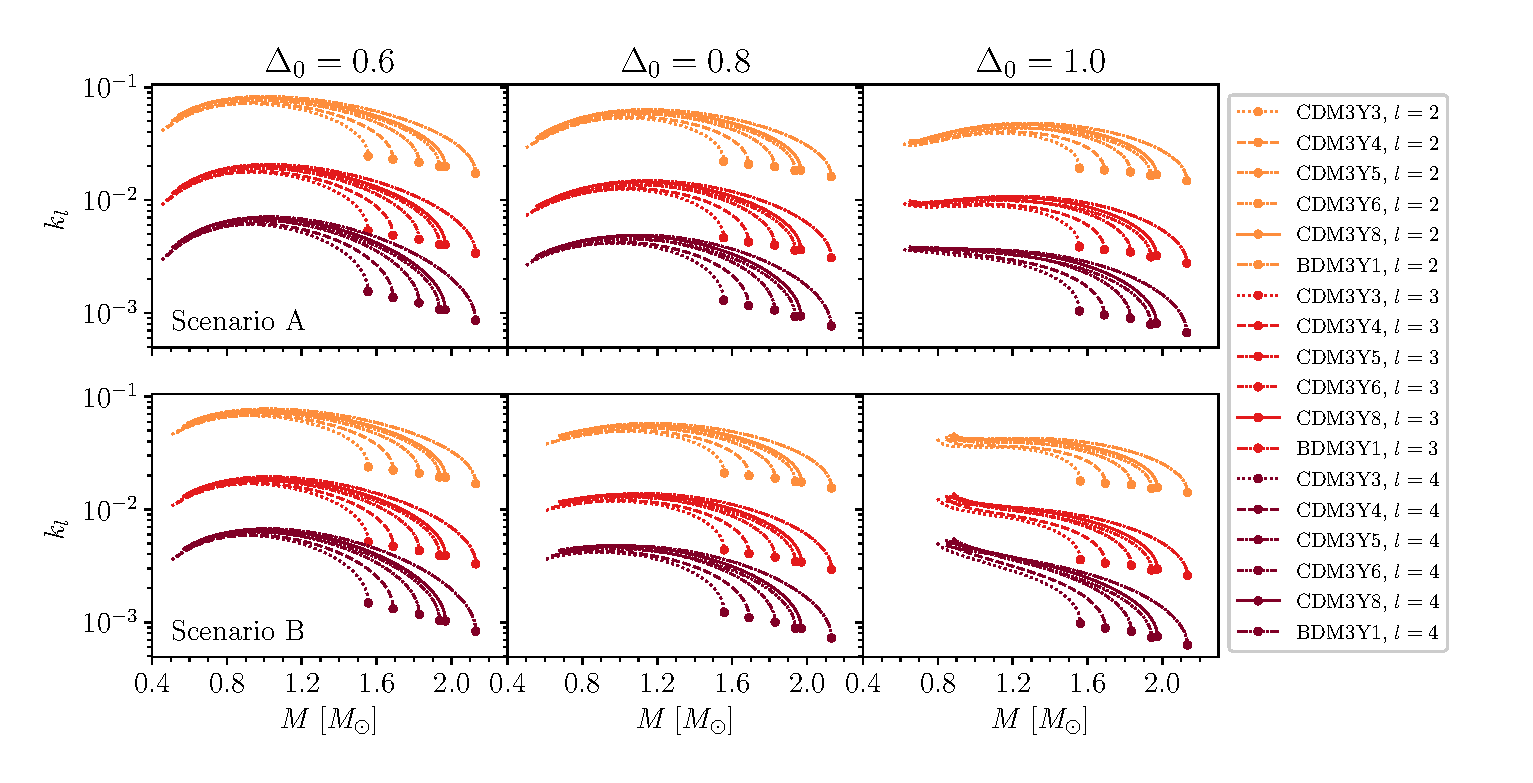
\includegraphics[width=\textwidth]{fig/kl.eps}
        \caption{\gls{GE} tidal Love number at $l$\textsuperscript{th} order $k_l$ as function of magnetar mass computed with 4 density-dependent \gls{NN} interaction versions at different spin polarizations. The dot at the end of each line represents the maximum gravitational mass $M$ of the magnetar generated by the corresponding \gls{EoS}.}
        \label{fig:kl}
\end{figure} 
\begin{figure}[ht!]
    \centering
    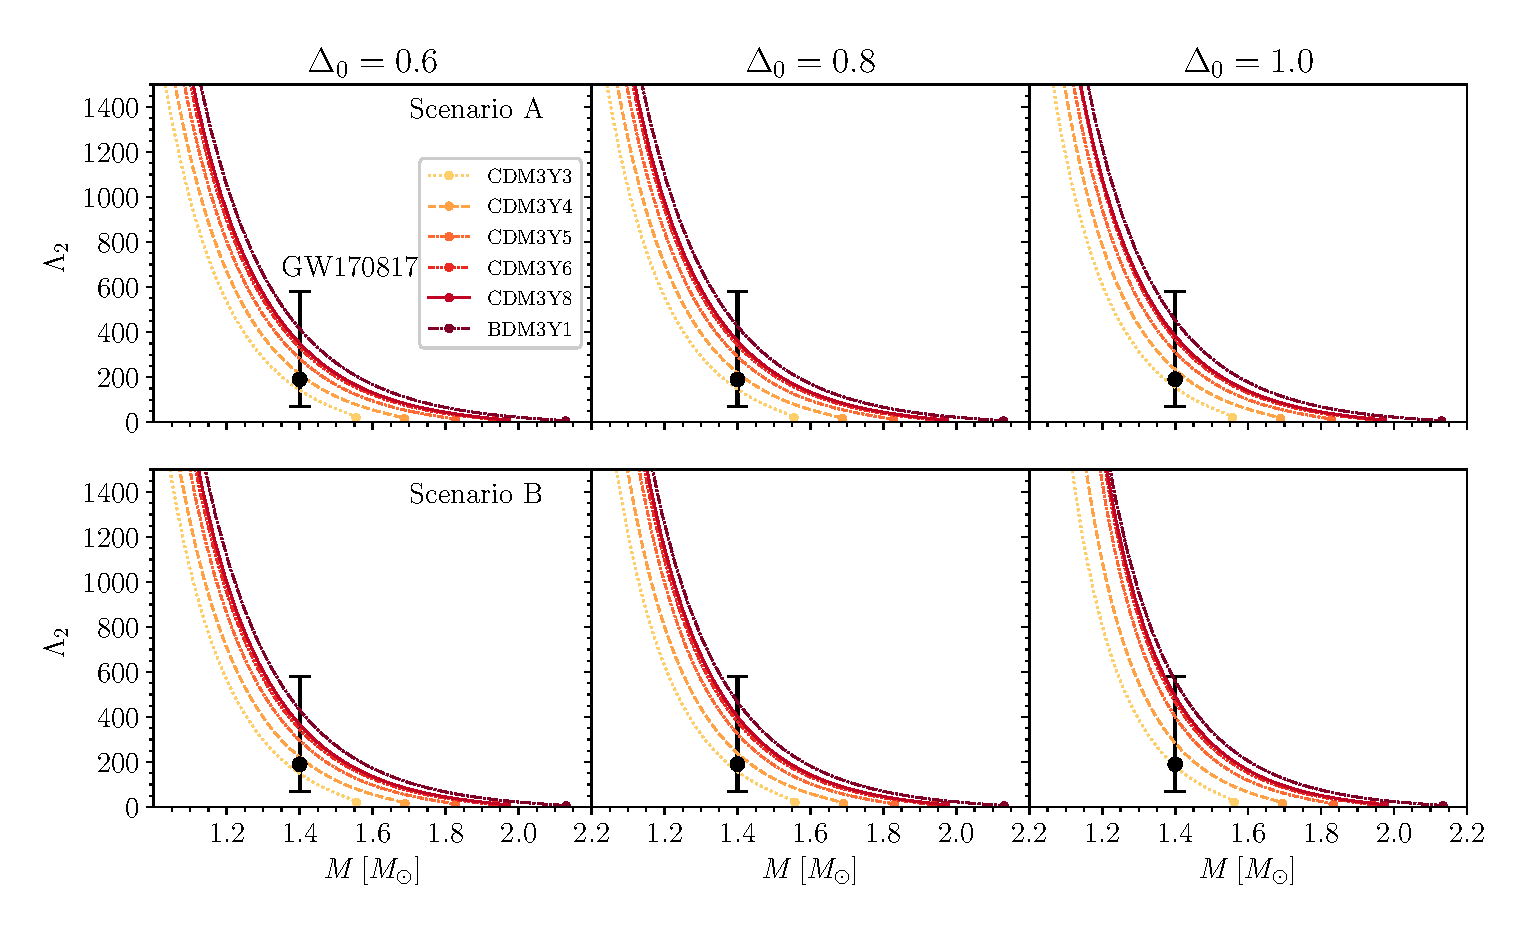
\includegraphics[width=\textwidth]{fig/Lambda2.eps}
    \caption{Dimensionless \gls{GE} tidal deformability parameter of 2\textsuperscript{nd} order $\Lambda_2$ of different CDM3Y$n$ models with varying $\Delta$. The vertical bar is the empirical tidal deformability constraint $\Lambda_2 \approx 190_{-120}^{+390}$ at $1.4M_\odot$, obtained from the Bayesian analysis of GW170817 data with 90\% confidence level \citep{abbott2018gw170817}.}
    \label{fig:Lambda2}
\end{figure} 
The results for \gls{GE} tidal Love number's dependence on \gls{NS}'s gravitational mass arose from 4 versions of the \gls{EoS} are shown in Figure \ref{fig:kl}. Similar to \cite{perot2021role}, in this result, it is clear that the higher the order $l$, the less impactful the Love number $k_l$ is for the tidal properties of the \gls{NS}, i.e. $k_l$ tends to be smaller by an order of magnitude than $k_{l-1}$, as expected from the multipole expansion. The 2\textsuperscript{nd} order is consequently dominant compared to the others. Between two scenarios A and B, at partial polarization of $\Delta_0 = 0.6$, the difference in $k_l$ of the same order is insignificant, except for the small difference in the low mass section. On the other hand, for the case of higher spin polarity in the \gls{NS} surface, the results are much more distinguishable, as the computation with scenario B gives rise to a ``steeper'' curve of $k_l$. Furthermore, in general, the maximum values of $k_l$ are at the common gravitational mass $M$ at all orders computed so far, and this value of $M$ seems to only depends on the value of $\Delta_0$, where the position of maximum $k_l$ tends to be shifted to a higher $M$ as $\Delta_0$ increases. Among these tidal parameters, the only one that has been constrained by far is the dominant 2\textsuperscript{nd} order Love number, which is investigated through the closely related dimensionless tidal deformability parameter of second order $\Lambda_2$ \eqref{eq:Lambda} and whose results are given in Figure \ref{fig:Lambda2}. In the study of \cite{abbott2018gw170817}, the range of $\Lambda_2$ is accepted to be $\Lambda_2 \approx 190^{+390}_{-120}$ at $M=1.4M_\odot$. It is interesting to note that for all cases in this study, this constraint tolerates all \glsplural{EoS} and scenarios, as well as the value of $\Delta_0$, thus no further exclusion can be done with this parameter. It's worth mentioning that the nuclear incompressibility $K$ plays a significant role in determining the tidal deformability $\Lambda_2$ as when $K$ varies from version to version (CDM3Y4 to CDM3Y8), the value of $\Lambda_2$ increases by $\approx 3$ times for the scenario A of $\Delta_0 = 0.6$ case, the same can be said for the different configuration of $\Delta(n_b)$. Testing the values of $k_l$ at higher orders can also be done by evaluating the tidal correction of the \gls{GW} waveform from inspiralling \glsplural{NS} within the PN theory, i.e. the \gls{GE} contribution of order $(2l+1)$PN to the phase of \gls{GW} signal is \citep{perot2021role, yagi2014multipole}
\begin{equation}
    \Psi_l = - \sum^{2}_{i=1} \left[ \frac{5}{16} \frac{(2l-1)!! (4l+3)(l+1)}{(4l-3)(2l-3)} \Lambda_{l,i} X_i^{2l-1} x^{2l - 3/2} + \frac{9}{16} \delta_{l2} \Lambda_{2, i} \frac{X_i^4}{\eta} x^{5/2} \right] + \mathcal{O}(x^{2l-1/2})
\end{equation}
where $i=1,\,2$ is the index distinguishing the two \glsplural{NS} of the system, $x=\left( G\pi Mf/c^3 \right)^{2/3}$, $f$ is the \gls{GW} signal frequency, $M=M_1 + M_2$, $X_i = M_i/M$ and $\eta = M_1 M_2/M^2$.

The gravito-magnetic tidal Love numbers $j_l$ contribute more weakly to the \gls{GW} phase compared to that of their \gls{GE} counterpart, as the \gls{GM} terms only appear from higher orders of $(2l+2)$PN, where the first correction at 6PN is given by \citep{perot2021role,yagi2017erratum}
\begin{equation}
    \tilde{\Psi}_2 = \sum^{2}_{i=1} \frac{5}{224} \sigma_{2,i} \frac{X_i^4}{\eta} \left( X_i - 1037X_j \right)x^{7/2} + \mathcal{O}(x^{9/2})
\end{equation}
\begin{figure}[ht!]
        \centering
        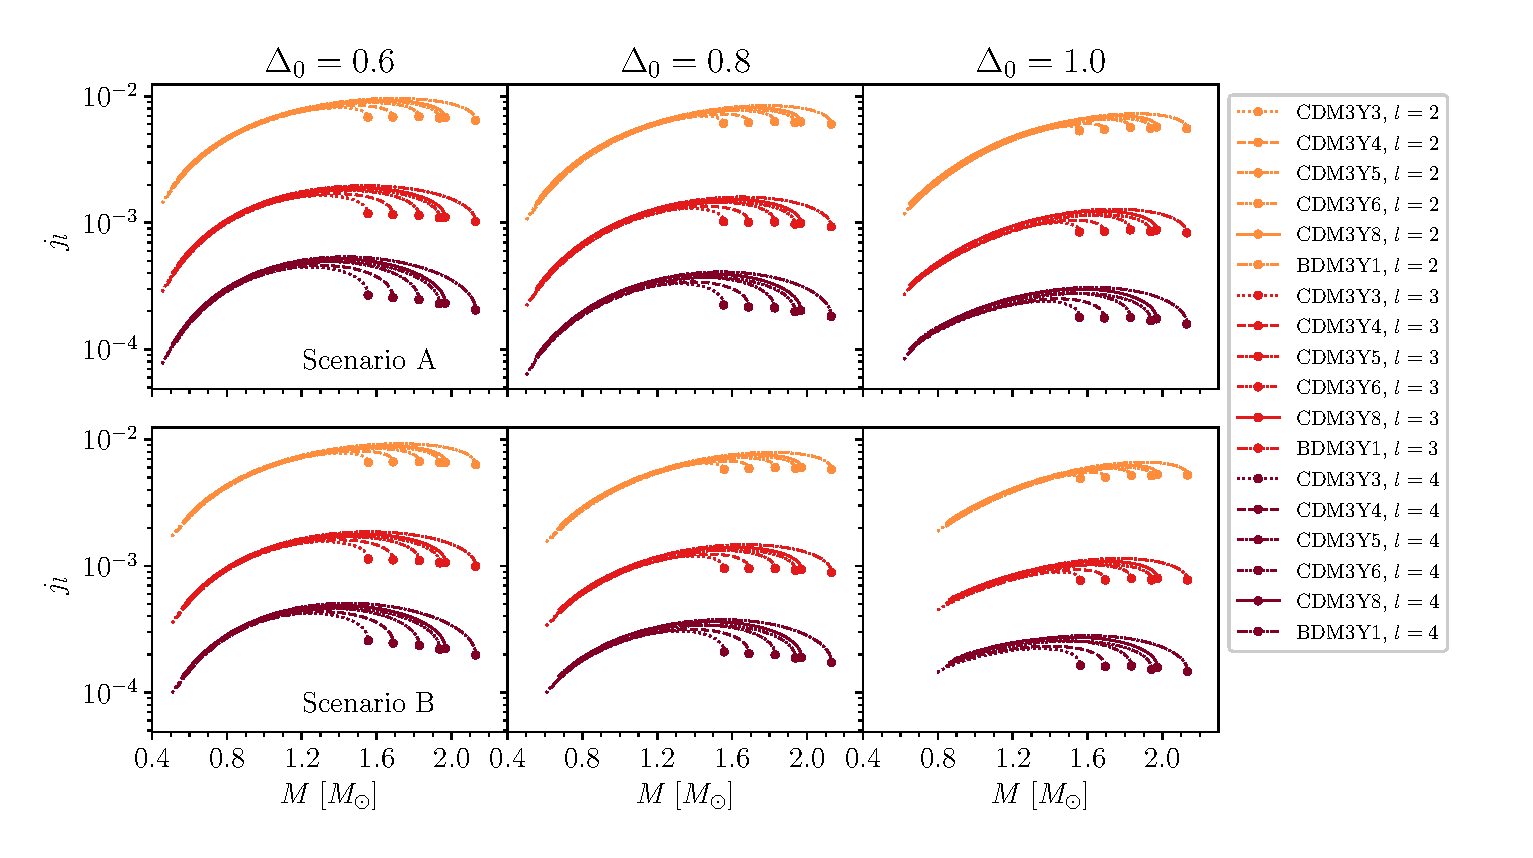
\includegraphics[width=\textwidth]{fig/jl_stat.eps}
        \caption{\gls{GM} tidal Love number at $l$\textsuperscript{nd} order $j_l$ as function of \gls{NS} mass computed with CDM3Y$n$ models of \emph{strictly static fluid} at different polarizations.}
        \label{fig:jl_stat}
\end{figure} 
\begin{figure}[ht!]
        \centering
        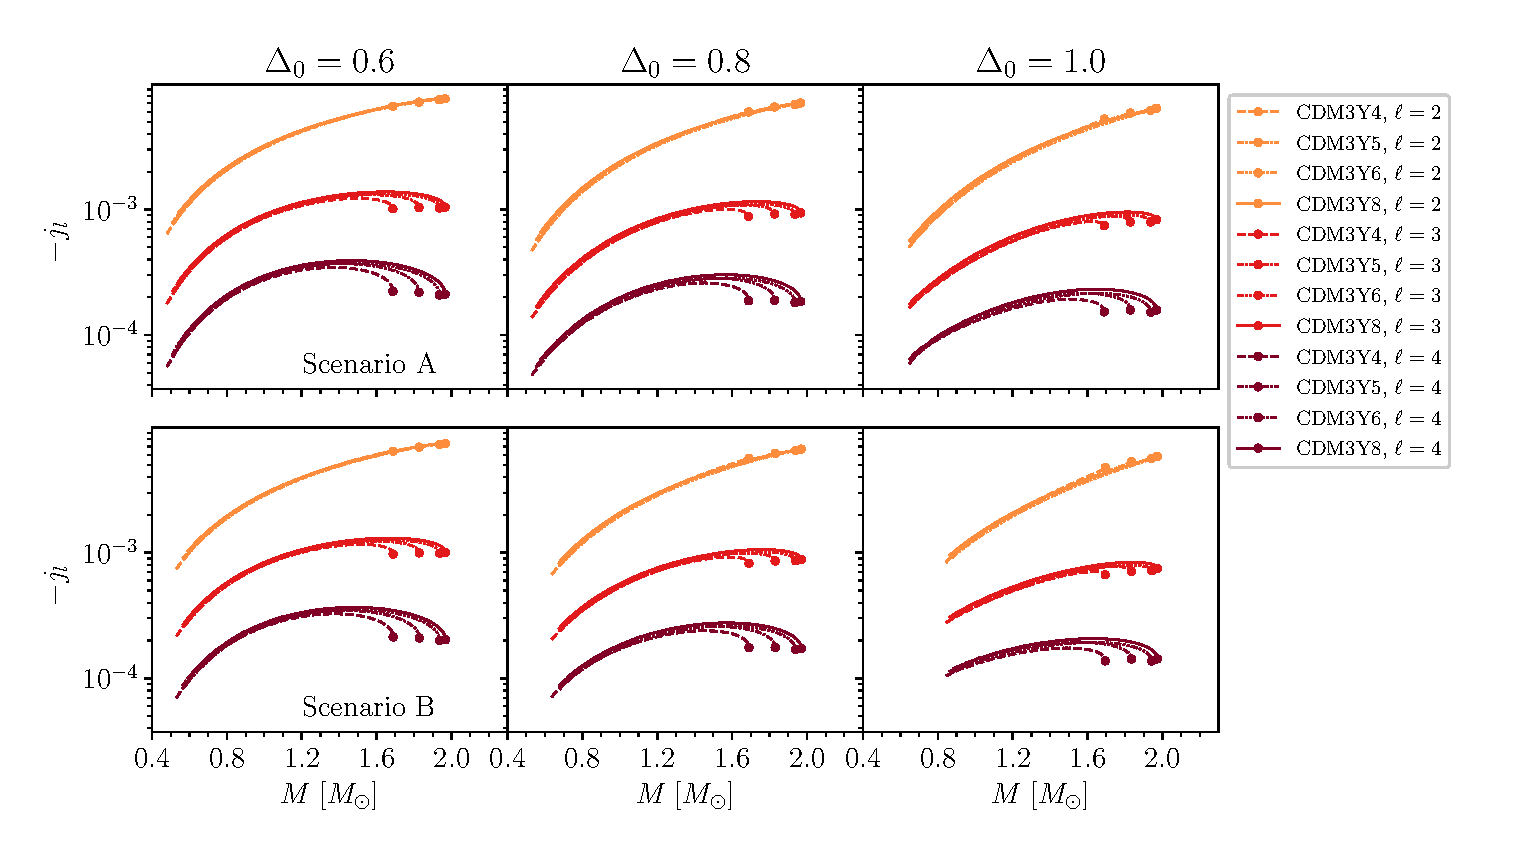
\includegraphics[width=\textwidth]{fig/jl_irrot.eps}
        \caption{\gls{GM} tidal Love number at $l$\textsuperscript{nd} order $j_l$ as function of \gls{NS} mass computed with CDM3Y$n$ models of \emph{irrotational fluid} at different polarizations.}
        \label{fig:jl_irrot}
\end{figure} 
The \gls{GM} tidal Love numbers of second, third and fourth order computed with 4 different \glsplural{EoS} are shown in Figure \ref{fig:jl_stat} for strictly static fluid and \ref{fig:jl_irrot} for irrotational fluid. Apart from the same trends as the \gls{GE} tidal Love numbers discussed previously, the \gls{GM} Love numbers' values do not have much variation as $\Delta_0$ increases in each scenario, as the shape of each curves in Figure \ref{fig:jl_stat} doesn't differ far from each others except for the difference in range of gravitational mass $M$. The value of $j_l$ corresponding to the \gls{GM} pertubation of irrotational fluid (Figure \ref{fig:jl_irrot}), on the other hand, stands out from the other two types of Love numbers, where its value is completely negative, albeit having the same magnitude as that of static fluid, this type of fluid motion is stated to be more realistic in this case due to it being driven by the tides \citep{perot2021role,pani2018magnetic}. In this case, the lines traced by each interation appear to reach maximum value at the maximum $M$ at the leading terms only, rather than having a local maxima in between. The dominance of the 2\textsuperscript{nd} order terms are clear in all cases, where the difference of around one order of magnitude is maintained. Notably, for the \gls{GM} terms corresponding with each \gls{NN} interaction, at higher order $l$, the \gls{NS} mass at maximum $j_l$ seems to become smaller. One more interesting result is that the magnitudes of $j_l$ for two types of fluid are also comparable but is smaller than their \gls{GE} counterpart by one order of magnitude, similar to the conclusion reached by \cite{perot2021role}.
